\documentclass{article}
\usepackage{amsmath}
\usepackage[mathletters]{ucs}
\usepackage[utf8x]{inputenc}
\usepackage[margin=1.5in]{geometry}
\usepackage{enumerate}
\newtheorem{theorem}{Theorem}
\usepackage[dvipsnames]{xcolor}
\usepackage{pgfplots}
\setlength{\parindent}{0cm}
\usepackage{graphics}
\usepackage{graphicx} % Required for including images
\usepackage{subcaption}
\usepackage{bigintcalc}
\usepackage{pythonhighlight} %for pythonkode \begin{python}   \end{python}
\usepackage{appendix}
\usepackage{arydshln}
\usepackage{physics}
\usepackage{tikz-cd}
\usepackage{booktabs} 
\usepackage{adjustbox}
\usepackage{mdframed}
\usepackage{relsize}
\usepackage{physics}
\usepackage[thinc]{esdiff}
\usepackage{fixltx2e}
\usepackage{esint}  %for lukket-linje-integral
\usepackage{xfrac} %for sfrac
\usepackage{hyperref} %for linker, må ha med hypersetup
\usepackage[noabbrev, nameinlink]{cleveref} % to be loaded after hyperref
\usepackage{amssymb} %\mathbb{R} for reelle tall, \mathcal{B} for "matte"-font
\usepackage{listings} %for kode/lstlisting
\usepackage{verbatim}
\usepackage{graphicx,wrapfig,lipsum,caption} %for wrapping av bilder
\usepackage{mathtools} %for \abs{x}
\usepackage[norsk]{babel}
\definecolor{codegreen}{rgb}{0,0.6,0}
\definecolor{codegray}{rgb}{0.5,0.5,0.5}
\definecolor{codepurple}{rgb}{0.58,0,0.82}
\definecolor{backcolour}{rgb}{0.95,0.95,0.92}

\lstdefinestyle{mystyle}{
    backgroundcolor=\color{backcolour},   
    commentstyle=\color{codegreen},
    keywordstyle=\color{magenta},
    numberstyle=\tiny\color{codegray},
    stringstyle=\color{codepurple},
    basicstyle=\ttfamily\footnotesize,
    breakatwhitespace=false,         
    breaklines=true,                 
    captionpos=b,                    
    keepspaces=true,                 
    numbers=left,                    
    numbersep=5pt,                  
    showspaces=false,                
    showstringspaces=false,
    showtabs=false,                  
    tabsize=2
}

\lstset{style=mystyle}
\author{Oskar Idland}
\title{MAT1120 Oblig 2}
\date{}
\begin{document}
\maketitle
\newpage

\section*{Oppgave 1}
  \[
  A = \begin{bmatrix}
   0 & 0 & \frac{1}{2} & 1 \\[1.1em]
   \frac{1}{3} & 0 & 0 & 0 \\[1.1em]
   \frac{1}{3} & \frac{1}{2} & 0 & 0 \\[1.1em]
   \frac{1}{3} & \frac{1}{2} & \frac{1}{2} & 0 \\ 
  \end{bmatrix}
  \]
Vi finner nullrommet ved å løse likningen 
\[
(A - I_4) \mathbf{x} = \mathbf 0 
\]
Da får vi at nullrommet har en basis 
\[
\mathbf{x} = \begin{pmatrix}
 \frac{4}{3} \\[.5em]
 \frac{4}{9} \\[.5em] 
 \frac{2}{3} \\[.5em]
 1 \\
\end{pmatrix}
\]
For å finne score vektoren må vi sørge for at summen $ s $ av elementene er lik 1. Vi summerer da alle verdiene og deler $ \mathbf{x} $ på denne summen
\[
s = \frac{4}{3} + \frac{4}{9} + \frac{2}{3} + 1 = \frac{31}{9}
\]


Score vektoren blir da 
\[
\frac{9}{31} \mathbf{x} = 
\begin{pmatrix}
\frac{12}{31}\\[.5em]
\frac{4}{31}\\[.5em]
\frac{6}{31}\\[.5em]
\frac{9}{31}
\end{pmatrix} = 
\frac{1}{31} 
\begin{pmatrix*}
 12 \\
 4 \\
 6 \\
 9 \\
\end{pmatrix*}
\]
Nå har hvert dokument en score og de kan rangeres 

\begin{center}
    \begin{tabular}{|c|*{1}{c|}}
        \hline
        Dokument & Rank \\
        \hline
        1 & 1\\
        \hline
        4 & 2 \\
        \hline
        3 & 3\\
        \hline
        2 & 4\\
        \hline
        \end{tabular}
\end{center}

\section*{Oppgave 2}

\[
A = 
\begin{bmatrix*}[r]
 0 & 0 & 0 & 0 & 1 \\
 0 & 0 & \frac{1}{2} & 1 & 0 \\
 0 & 0 & 0 & 0 & 0 \\
 0 & 1 & \frac{1}{2} & 0 & 0 \\
 1 & 0 & 0 & 0 & 0 \\
\end{bmatrix*}
\]

Vi finner nullrommet ved å løse likningen 
\[
(A - I_5) \mathbf{x} = \mathbf 0 
\]

\[
\begin{bmatrix*}[r]
 1 & 0 & 0 & 0 & -1 & 0 \\
 0 & 1 & 0 & -1 & 0 & 0 \\
 0 & 0 & 1 & 0 & 0 & 0 \\
 0 & 0 & 0 & 0 & 0 & 0 \\

\end{bmatrix*}
\]

Dette likningsettet har ingen løsning og derfor har ikke matrisen en unik score vektor. 

\section*{Oppgave 3}
Begge matriser er stokastiske ettersom alle søylene inneholder ikke-negative elementer. For å se om den første matrisen er regulær må vi finne en eksponent som gjør at alle elementene er positive tall

\[
  A = \begin{bmatrix}
   0 & 0 & \frac{1}{2} & 1 \\[1.1em]
   \frac{1}{3} & 0 & 0 & 0 \\[1.1em]
   \frac{1}{3} & \frac{1}{2} & 0 & 0 \\[1.1em]
   \frac{1}{3} & \frac{1}{2} & \frac{1}{2} & 0 \\ 
  \end{bmatrix}
  \]

\[
A^{4} = \begin{bmatrix}
\frac{1}{3} & \frac{3}{8} & \frac{11}{24} & \frac{5}{12}\\[1.1em]
\frac{5}{36} & \frac{1}{12} & \frac{1}{12} & \frac{1}{6}\\[1.1em]
\frac{2}{9} & \frac{5}{24} & \frac{1}{6} & \frac{1}{6}\\[1.1em]
\frac{11}{36} & \frac{1}{3} & \frac{7}{24} & \frac{1}{4}
\end{bmatrix}
\]
Vi ser at hvis den første matrisen får 4 som eksponent blir alle elementene positive og den er dermed regulær.
Vi prøver så dette på den andre matrisen

\[
B =
\begin{bmatrix}
 0 & 0 & 0 & 0 & 1 \\
 0 & 0 & \frac{1}{2} & 1 & 0 \\
 0 & 0 & 0 & 0 & 0 \\
 0 & 1 & \frac{1}{2} & 0 & 0 \\
 1 & 0 & 0 & 0 & 0 \\
\end{bmatrix}
\]
\[
B^{2} = \begin{bmatrix}1 & 0 & 0 & 0 & 0\\0 & 1 & \frac{1}{2} & 0 & 0\\0 & 0 & 0 & 0 & 0\\0 & 0 & \frac{1}{2} & 1 & 0\\0 & 0 & 0 & 0 & 1\end{bmatrix} = 
B^{4} = \begin{bmatrix}1 & 0 & 0 & 0 & 0\\0 & 1 & \frac{1}{2} & 0 & 0\\0 & 0 & 0 & 0 & 0\\0 & 0 & \frac{1}{2} & 1 & 0\\0 & 0 & 0 & 0 & 1\end{bmatrix}
\]
Her ser vi et klart mønster hvor matrisen opphøyd i $ n $ er en speilet versjon av matrisen opphøyd i $ n+1 $ om midterste søyle og vil dermed aldri opppnå kravet om at alle elementer er positive. Denne matrisen er dermed ikke regulær

  
  
\section*{Oppgave 7}

Vi kjører koden og får følgende matrise:
\[
A=
\begin{bmatrix*}[r]
 0 & \frac{1}{2} & 0 & 0 & \frac{1}{4} \\[1.1em]
 \frac{1}{2} & 0 & \frac{1}{2} & 0 & \frac{1}{4} \\[1.1em]
 0 & 0 & 0 & 0 & \frac{1}{4} \\[1.1em]
 0 & 0 & 0 & 0 & \frac{1}{4} \\[1.1em]
 \frac{1}{2} & \frac{1}{2} & \frac{1}{2} & 1 & 0 \\
\end{bmatrix*}
\]

Dette tilsvarer følgende web
\begin{figure}[h!]
  \centering
  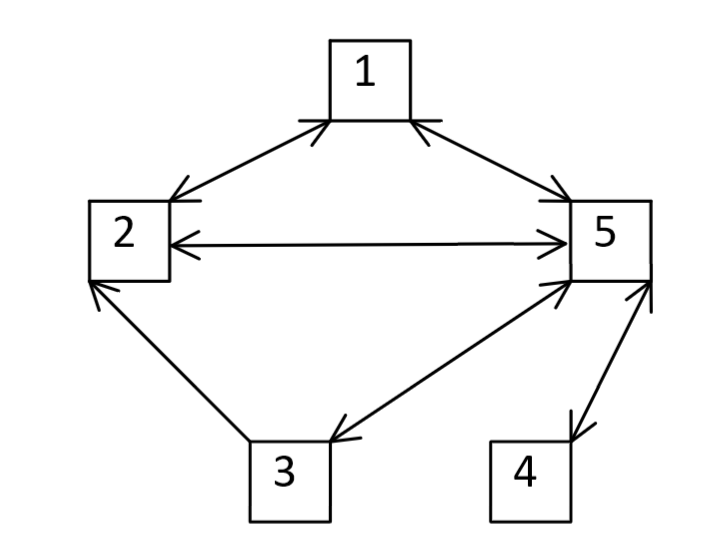
\includegraphics[scale = .7]{web.png}
  \caption{Web som tilsvarer matrisen gitt over}
  \label{fig: web}
\end{figure}

\newpage
\section*{Oppgave 8-10}
Ved bruk av en python funskjon ser vi at score vektoren til $ A $ blir følgende

\[
≈
\begin{pmatrix*}[r]
 0.21 \\
 0.24 \\
 0.10 \\
 0.10 \\
 0.36 \\
\end{pmatrix*}
\]

Ved bruk av python funksjonen rankingApprox rett etter den nøyaktige løsningen ser vi at approksimasjonen er helt presis for vårt anntall desimaler.  
\begin{figure}[h!]
  \centering
  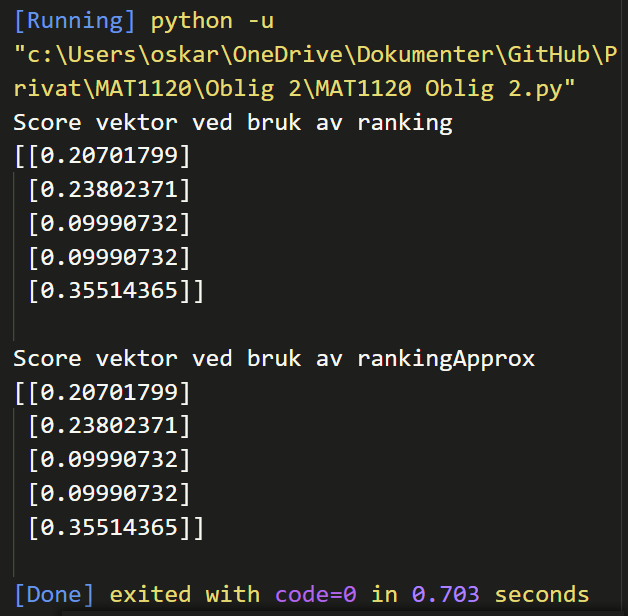
\includegraphics[scale = .7]{rank_rankapprox.png}
  \caption{Output fra kode ved å kjøre funksjonene ranking og rankingApprox}
  \label{fig:figure1}
\end{figure}


\newpage
\section*{Kode}
\lstinputlisting{MAT1120 Oblig 2.py}

\end{document}
